\documentclass[11pt]{article}
\usepackage[T1]{fontenc}
\usepackage{lmodern,microtype}
\usepackage[margin=1.08in]{geometry}
\usepackage{amsmath,amssymb,amsthm,mathtools}
\usepackage{enumitem}
\usepackage{tikz}
\usepackage[colorlinks=true,linkcolor=blue,citecolor=blue,urlcolor=blue]{hyperref}
\hypersetup{pdftitle={Interior regularity of planar Mumford--Shah minimizers},pdfauthor={OpenAI}}
\pdfinfoomitdate=1
\pdftrailerid{}
\pdfsuppressptexinfo=15
\newtheorem{theorem}{Theorem}[section]
\newtheorem{proposition}[theorem]{Proposition}
\newtheorem{lemma}[theorem]{Lemma}
\newtheorem{corollary}[theorem]{Corollary}
\theoremstyle{definition}
\newtheorem{definition}[theorem]{Definition}
\newtheorem{remark}[theorem]{Remark}
\numberwithin{equation}{section}
\title{Interior regularity of planar\\Mumford--Shah minimizers}
\author{OpenAI}
\date{September 24, 2026}
\begin{document}
\maketitle
\begin{abstract}
We prove the interior regularity assertion of the planar Mumford--Shah
conjecture for reduced absolute minimizers with bounded fidelity data.
Every interior point of the closed discontinuity set has a neighborhood
consisting of a $C^{1,\alpha}$ arc, an arc ending at that point, or three
such arcs meeting at $120$ degrees. Only finitely many global connected
components meet any relatively compact open set.
\end{abstract}
\tableofcontents
\section{Introduction}
The planar Mumford--Shah problem balances smoothness of a function against
the length of a set across which it may jump.  Its regularity conjecture
predicts that, in the interior, this set consists of regular arcs with only
free endpoints and triple junctions.  We prove this interior conclusion
for the absolute comparison problem defined below.  The proof also gives
local finiteness of the global connected components of the closed set.

\subsection{The variational problem}
\label{sec:problem}
Let $\Omega\subset\mathbb R^2$ be a bounded Lipschitz domain and let
$g\in L^\infty(\Omega)$ be real-valued.  We write $\mathcal H^1$ for
one-dimensional Hausdorff measure.  A pair $(u,K)$ is \emph{admissible} if
\[
 K\subset\Omega\text{ is relatively closed},\qquad
 \mathcal H^1(K)<\infty,\qquad
 u\in L^2(\Omega),\qquad
 u|_{\Omega\setminus K}\in W^{1,2}(\Omega\setminus K).
\]
No rectifiability of $K$ is assumed.  Values of $u$ on $K$ do not affect
any integral.  For open $V\subset\Omega$, set
\begin{equation}\label{eq:original-energy}
 \mathcal F_g(u,K;V)
 =\int_{V\setminus K}|\nabla u|^2\,dx
   +\mathcal H^1(K\cap V)+\int_V|u-g|^2\,dx.
\end{equation}
Here and below, $V\Subset\Omega$ means that $\overline V$ is a compact
subset of $\Omega$.

An admissible pair is an \emph{absolute minimizer} if, for every open
$V\Subset\Omega$ and every admissible $(w,L)$ with
\begin{equation}\label{eq:compact-comparison}
 (L\mathbin{\triangle}K)\cup\operatorname{spt}(w-u)\Subset V,
\end{equation}
one has $\mathcal F_g(u,K;V)\le\mathcal F_g(w,L;V)$.
The support of a function is understood in the essential sense.
The pair is \emph{reduced} if
\begin{equation}\label{eq:reduced}
 K=\operatorname{spt}_{\Omega}(\mathcal H^1\!\llcorner K).
\end{equation}
Equivalently, every disk centered at a point of $K$ and compactly
contained in $\Omega$ contains a positive length of $K$.  This removes
closed additions of zero length that have no effect on the energy.

\subsection{Main theorem}
\begin{theorem}\label{thm:main}
Let $(u,K)$ be a reduced absolute minimizer of
\eqref{eq:original-energy} in a bounded Lipschitz domain
$\Omega\subset\mathbb R^2$, with $g\in L^\infty(\Omega)$.
Every $x\in K$ has an interior neighborhood in which $K$ has one of the
following forms, with $C^{1,\alpha}$ arcs for some $\alpha>0$:
\begin{enumerate}[label=\textup{(\roman*)},nosep]
 \item a single embedded arc with $x$ in its interior;
 \item a single embedded arc ending at $x$;
 \item three embedded arcs meeting only at $x$, with pairwise angles
       $120$ degrees.
\end{enumerate}
Moreover, for every open $U\Subset\Omega$,
\begin{equation}\label{eq:component-finiteness}
 \#\{C\in\pi_0(K):C\cap U\ne\varnothing\}<\infty,
\end{equation}
where $\pi_0(K)$ denotes the set of global connected components of $K$.
\end{theorem}

The theorem gives the interior regularity conclusion of the planar
Mumford--Shah conjecture.  The compact-set qualification is essential to
the scope of the statement: we make no assertion about finiteness up to
$\partial\Omega$.  The components counted in
\eqref{eq:component-finiteness} are components of $K$, rather than of a
truncation $K\cap U$ or of its complement.

The geometric conclusion also gives an endpoint integrability estimate for
the gradient.  Corollary~\ref{cor:weak-l4} proves
\[
 \nabla u\in L^{4,\infty}_{\mathrm{loc}}(\Omega),
 \qquad \nabla u\in L^p_{\mathrm{loc}}(\Omega)\quad(0<p<4).
\]
Here weak $L^4$ means that the area of the gradient superlevel set
$\{|\nabla u|>t\}$ in each relatively compact region is bounded by a
constant times $t^{-4}$.  The exponent reflects the inverse-square-root
gradient at a crack tip.

\subsection{History and related work}
Mumford and Shah introduced their functional as a model for image
segmentation \cite{mumford_shah1989}. The fidelity term keeps the
reconstruction close to the observed image, the Dirichlet term favors
smooth variation within regions, and the length term penalizes the edges
between them. Their regularity conjecture asks whether minimization itself
forces the simple interior geometry suggested by this model. Deriving that
geometry requires controlling arbitrary finite-length discontinuity sets,
including possible accumulation of their components.

The theory of special functions of bounded variation provides the weak
variational framework for this problem. De Giorgi and Ambrosio introduced
this free-discontinuity setting \cite{degiorgi_ambrosio1988}, and Ambrosio
developed the compactness and existence theory
\cite{ambrosio1989,ambrosio1990}. The existence and essential-closure results
of De Giorgi, Carriero, and Leaci, together with the Dirichlet theory of
Carriero and Leaci, connect weak minimizers with the classical closed-set
formulation \cite{degiorgi_carriero_leaci1989,carriero_leaci1990}.
We use this connection to establish rectifiability of the given set before
applying geometric regularity theory. The underlying bounded-variation
extension and trace calculus are treated systematically in
Ambrosio, Fusco, and Pallara \cite{ambrosio_fusco_pallara2000}.

Bonnet introduced the planar blow-up and monotonicity approach and
classified global minimizers with connected crack set
\cite[Theorems~2.2, 3.1, and~4.1]{bonnet1996}.
Regular-arc and partial-regularity theory was developed independently by
David and by Ambrosio, Fusco, and Pallara
\cite{david1996,ambrosio_fusco_pallara1997}; David also established the
triple-junction theory and developed its quantitative geometric framework
\cite{david1996,david2005}. Bonnet and David proved global minimality of
the crack tip and classification when the part outside one connected
component is bounded \cite{bonnet_david2001}. David and L\'eger proved
that a global minimizer whose crack disconnects the plane must be a line
or a $120$-degree triod \cite[Corollary~9.16]{david_leger2002}.
In the generalized-limit formulation recalled below, these classification
results leave the possible bounded components of a limiting crack as the
remaining obstruction. Higher-integrability theorems of De Lellis--Focardi
in the plane and De Philippis--Figalli in arbitrary dimension supplied
further control of the exceptional set
\cite{delellis_focardi2013,dephilippis_figalli2014}.

Regularity at an endpoint requires additional analysis. Work of Andersson
and Mikayelyan on crack tips \cite{andersson_mikayelyan2019} was revisited
by De Lellis, Focardi, and Ghinassi
\cite{delellis_focardi_ghinassi2021,delellis_focardi_ghinassi_erratum}.
For the bounded measurable fidelity datum used here, we invoke the exact
geometric regularity and compactness statements in the monograph of
De Lellis and Focardi \cite{delellis_focardi2025}. Recent work of Labourie
and Lemenant establishes at most three limiting values and controls local
components of the complement \cite{labourie_lemenant2026}. The component
count in Theorem~\ref{thm:main} concerns the closed crack set itself.

Deangelis's recent preprint gives a proof of the global classification and
the resulting interior arc, endpoint, and triple-junction structure
\cite[Theorems~1.1 and~3.4]{deangelis2026}. His compact-translation
argument combines relaxed second variations, equality in a planar Hodge
identity, and holomorphic rigidity. Both arguments use whole-plane
projections and value variations with independently prescribed one-sided
traces on a regular arc; see \cite[Section~3.2]{deangelis2026}.
The proof below obtains a scalar harmonic interaction from finite
translations and an explicit cutoff at infinity; minimality forces this
interaction to be constant.

\subsection{Proof strategy}
We first pass from the stated finite-length formulation to a locally
bounded, rectifiable minimizing pair.  The reduction uses clipping inside
disks and a Dirichlet comparison with smooth approximations of the boundary
trace; it preserves the original pair.

At an interior point $x$, the rescaled closed sets $(K-x)/r_j$, with
$r_j\downarrow0$, have global generalized limits $H$.  These are limits
of absolute minimizers, with additive constants in each complementary
component recorded as part of the limiting data.  The established
compactness and rigidity theorems reduce their classification to excluding
a bounded component when $\mathbb R^2\setminus H$ is connected.  In this
case the limit function $v$ is an absolute minimizer of the zero-fidelity
energy on the whole plane.

A bounded component can be enlarged to a compact piece $A\subset H$ at
positive distance from $B=H\setminus A$.  We split the gradient of $v$
into a field carrying the jumps across $A$ and the gradient of a harmonic
potential that extends through $A$.  Translating $A$ leaves its length unchanged.  The
interaction between these two fields is harmonic in the translation
parameter; minimality forces it to be constant.  Independent changes in
the jump values along a regular subarc of $A$ then force this harmonic
potential to be affine.  The energy growth bound makes its gradient zero;
the value-variation identity then makes the remaining field zero.
Removing $A$ saves positive length, a contradiction.

The known classification now gives only a line, a halfline or three rays
for a nonempty blow-up set.  Epsilon regularity transfers these models to
the original minimizer.  Finally, a finite cover of $K\cap\overline U$ by
connected model neighborhoods proves \eqref{eq:component-finiteness}.
The resulting absence of irregular points also yields the local weak-$L^4$
gradient estimate through the De Lellis--Focardi equivalence.

The reduction occupies Section~\ref{sec:initial-reduction}, and
Section~\ref{sec:known-facts} records the compactness and regularity
results used below.  Sections~\ref{sec:isolation} and~\ref{sec:compact-piece} establish
the compact-piece exclusion.  Section~\ref{sec:assembly} completes the
classification, proves Theorem~\ref{thm:main}, and derives the weak-$L^4$
consequence.

\section{Reduction to rectifiable minimizers}
\label{sec:initial-reduction}

The admissible class in the problem does not assume that the closed set is
rectifiable or that the function is bounded.  We establish both properties
locally before using the classical regularity theory.  The essential point is
that a portion of the closed set which carries no jump can be removed by a
Dirichlet replacement, with an arbitrarily small error on the boundary of the
replacement disk.

We use the following standard notation.  A function is in $BV(W)$ if its
distributional derivative is a finite vector-valued Radon measure on $W$.
Its derivative decomposes into an absolutely continuous part, a jump part,
and a Cantor part.  The jump part is concentrated on the approximate jump
set $J_u$, where two distinct one-sided approximate limits exist across a
line.  The space $SBV(W)$ consists of the $BV$ functions whose Cantor part
vanishes.  We use two basic facts from the $BV$ structure theorem: $J_u$ is
countably $1$-rectifiable (covered, up to a set of zero length, by
countably many Lipschitz images of intervals), and the Cantor part gives zero mass to every set
of $\sigma$-finite $\mathcal H^1$ measure
\cite[Theorem~3.78 and Proposition~3.92(c)]{ambrosio_fusco_pallara2000}. The same notation with the
subscript ${\rm loc}$ requires these properties on relatively compact
open subsets.

\begin{proposition}[Reduction to a rectifiable pair]
\label{prop:initial-reduction}
Let $\Omega\subset\mathbb R^2$ be bounded and open, let
$g\in L^\infty(\Omega)$, and let $(u,K)$ be an admissible absolute
minimizer for $\mathcal F_g$ as defined in Section~\ref{sec:problem}.  In particular,
$K$ is relatively closed, $\mathcal H^1(K)<\infty$, and
$u\in L^2(\Omega)\cap W^{1,2}(\Omega\setminus K)$; no rectifiability
of $K$ is assumed.  Then
\[
 u\in L^\infty_{\rm loc}(\Omega)\cap SBV_{\rm loc}(\Omega),
 \qquad
 \mathcal H^1(K\setminus J_u)=0.
\]
The function satisfies $\Delta u=u-g$ on $\Omega\setminus K$ and has
there a $C^{1,\alpha}_{\rm loc}$ representative for every $\alpha\in(0,1)$.
If the pair is reduced, then
\begin{equation}
 K=\operatorname{spt}_{\Omega}(\mathcal H^1\!\llcorner J_u)
   =\overline{J_u}^{\,\Omega}.
 \label{eq:jump-support}
\end{equation}
Consequently, in the reduced case, on every smooth open set $W\Subset\Omega$, the restricted
pair is a reduced rectifiable absolute minimizer with bounded function.
\end{proposition}

The proof uses a standard Dirichlet theorem in the $SBV$ formulation.
We record the precise version needed here. Its weak minimizer is an
auxiliary replacement: essential closure will turn its jump set into an
admissible closed comparison set, allowing us to test the original pair.
For a disk $D$ and
$w\in C^1_c(\mathbb R^2)$, consider the functional
\begin{equation}
 \mathcal J_D(z)
 :=\int_D\bigl(|\nabla z|^2+|z-g|^2\bigr)\,dx
      +\mathcal H^1(J_z\cap\overline D)
 \label{eq:weak-dirichlet-energy}
\end{equation}
on $z\in SBV(\mathbb R^2)$ satisfying $z=w$ almost everywhere on
$\mathbb R^2\setminus D$.  Here $J_z$ is the jump set of the extension
to the whole plane.  In particular, a mismatch of boundary traces is
charged in \eqref{eq:weak-dirichlet-energy}.

\begin{lemma}[The smooth-data Dirichlet input]
\label{lem:dirichlet-input}
Let $D\subset\mathbb R^2$ be a disk, $g\in L^\infty(D)$, and
$w\in C^1_c(\mathbb R^2)$.  The problem
\eqref{eq:weak-dirichlet-energy} has a bounded minimizer $z$, and
\begin{equation}
 \mathcal H^1\bigl((\overline{J_z}\setminus J_z)
                  \cap\overline D\bigr)=0.
 \label{eq:dirichlet-essential-closure}
\end{equation}
In particular, $C:=\overline{J_z}\cap\overline D$ is compact and has
finite length, and $z$ belongs to $W^{1,2}_{\rm loc}$ on the complement
of $\overline{J_z}$.  On each relatively open portion of $\partial D$ disjoint from $C$,
its interior and exterior Sobolev traces agree almost everywhere.
\end{lemma}

This is the smooth-boundary, smooth-exterior-data case of the Dirichlet
existence and essential-closure theorem; see
\cite[Appendix~B]{delellis_focardi2025}, specifically
Theorem~B.3.1(c), Corollary~B.3.2(b), and Proposition~B.4.2(c).
The final two assertions also follow directly from the $SBV$ decomposition:
on an open set which misses the closed jump set there is no singular
derivative, while the absolutely continuous gradient is square integrable.
Across a jump-free boundary portion, apply this observation to the
whole-plane extension $z$, whose exterior value is $w$.

We explain explicitly why the boundary in
\eqref{eq:dirichlet-essential-closure} introduces no extra length.
The boundary density theorem supplies a positive lower bound for
$\mathcal H^1(J_z\cap B_r(x))/r$ as $r\downarrow0$ at points
$x\in\overline{J_z}\cap\partial D$.
Put $\mu=\mathcal H^1\!\llcorner J_z$ and
$\nu=\mathcal H^1\!\llcorner\partial D$.
The restriction of $\mu$ to the circle is
$\nu\!\llcorner(J_z\cap\partial D)$, while its remaining part is
singular with respect to $\nu$.  Differentiation of measures, together
with $\nu(B_r(x))/(2r)\to1$, gives
\[
 \frac{\mu(B_r(x))}{r}\longrightarrow0
 \quad\text{for $\mathcal H^1$-almost every }
 x\in\partial D\setminus J_z.
\]
This contradicts the boundary lower bound at any such point in the
closed jump set.  Hence the boundary portion of the difference in
\eqref{eq:dirichlet-essential-closure} is null.  The interior portion
is the usual interior essential-closure theorem.  No $C^1$ matching
of normal derivatives across $\partial D$ is used.

\begin{proof}[Proof of Proposition~\ref{prop:initial-reduction}]
We divide the argument into local boundedness, the $SBV$ extension,
and removal of excess length.

\smallskip
\noindent\emph{Step 1: circles with bounded traces.}
Variations $u+t\varphi$, with
$\varphi\in C^\infty_c(\Omega\setminus K)$, preserve the admissible
class and have compact support.  Their first variation gives
\[
 \int_{\Omega\setminus K}\nabla u\cdot\nabla\varphi
       +(u-g)\varphi\,dx=0.
\]
Thus $\Delta u=u-g$ off $K$.  In two dimensions, local
$W^{1,2}$ membership implies local $L^p$ membership for every finite
$p$.  Interior elliptic estimates therefore give
$u\in W^{2,p}_{\rm loc}(\Omega\setminus K)$ for all such $p$,
and hence the asserted $C^{1,\alpha}_{\rm loc}$ regularity.  We use
this representative off $K$ from now on.

Fix $q\in\Omega$.  For almost every radius $s$ with
$\overline B_s(q)\subset\Omega$, the following two properties hold:
\begin{equation}
 \Sigma_s:=K\cap\partial B_s(q)\text{ is finite},
 \qquad
 \int_{\partial B_s(q)\setminus K}
           (|u|^2+|\nabla u|^2)\,d\mathcal H^1<\infty.
 \label{eq:good-circle}
\end{equation}
The first assertion is Eilenberg's coarea inequality applied to the
$1$-Lipschitz distance map on a Borel set of finite $\mathcal H^1$
measure.  It requires no rectifiability.  The second follows from
polar integration.  To recall the elementary content of the first
inequality, cover a compact portion of $K$ by sets of diameter less
than $\delta$.  On each distance level, every $\delta$-separated
collection contains at most one point in each covering set.  The
image of a covering set lies in an interval no longer than its
diameter.  Integration over the levels, followed by refinement of
the covers and $\delta\downarrow0$, bounds the integral of the
level cardinality by the length of the covered set.

Call a disk satisfying \eqref{eq:good-circle} a good disk.
The circle minus $\Sigma_s$ consists of finitely many open arcs.
On each arc the restriction of $u$ is $C^1$, and its tangential
derivative is square integrable by \eqref{eq:good-circle}.
It is therefore a one-dimensional $W^{1,2}$ function and has finite
one-sided limits at the arc endpoints.  Its supremum is finite.
Taking the maximum over the finitely many arcs shows that the
circle trace $f$ is bounded.  If $\Sigma_s$ is empty, the same
conclusion follows from $W^{1,2}$ on the full circle.

\smallskip
\noindent\emph{Step 2: local boundedness by clipping.}
Fix a good disk $B=B_s(q)$ and choose
\[M>\max\{\|f\|_\infty,\|g\|_\infty\}.\]
Let $T_M(a)=\max\{-M,\min\{a,M\}\}$ and set
\[
 \widetilde u=T_M(u)\quad\text{in }B,
 \qquad \widetilde u=u\quad\text{in }\Omega\setminus B.
\]
The traces agree on $\partial B\setminus K$.  Sobolev gluing there,
together with the chain rule for $T_M$, shows that
$\widetilde u\in W^{1,2}(\Omega\setminus K)\cap L^2(\Omega)$.
Its difference from $u$ is supported in $\overline B$.
Choose an open $V$ with
$\overline B\Subset V\Subset\Omega$ and use
$(\widetilde u,K)$ in the defining comparison on $V$.
The Dirichlet term does not increase, and the fidelity term
strictly decreases wherever $|u|>M$ in $B$.
For example, on $\{u>M\}$ the decrease is
$(u-M)(u+M-2g)>0$.
Minimality therefore gives $|u|\le M$ almost everywhere in $B$.
Good disks exist with arbitrarily small radii about every point.
A finite cover of each compact subset of $\Omega$ proves
$u\in L^\infty_{\rm loc}(\Omega)$.

\smallskip
\noindent\emph{Step 3: the $SBV$ extension.}
We give the finite-ball extension argument underlying
\cite[Proposition~4.4]{ambrosio_fusco_pallara2000}; it requires no
rectifiability of the closed set.
Choose smooth open sets $W\Subset W'\Subset\Omega$.
The definition of $\mathcal H^1$ and compactness give finite
covers of $K\cap\overline W$ by open balls of radii $a_{ij}$ such
that
\[
 \max_i a_{ij}\longrightarrow0,
 \qquad \sum_i a_{ij}\le C(1+\mathcal H^1(K)),
 \qquad \overline{G_j}\subset W',
 \quad G_j:=\bigcup_i B_{a_{ij}}.
\]
Their areas tend to zero and their perimeters satisfy
$\operatorname{Per}(G_j)\le2\pi\sum_i a_{ij}$.
Moreover, $\partial G_j\cap W$ misses $K$, since the open union
covers $K\cap\overline W$.
Set $u_j=0$ on $G_j\cap W$ and $u_j=u$ elsewhere in $W$.
Integration by parts along the exposed circular arcs gives
\[
 |Du_j|(W)
 \le\int_{W\setminus K}|\nabla u|\,dx
      +2\pi\|u\|_{L^\infty(W')}\sum_i a_{ij}.
\]
This estimate can equivalently be read as the finite-perimeter
product rule.  Test fields compactly supported in $W$ produce no
term on $\partial W$.
Since $u_j\to u$ in $L^1(W)$, lower semicontinuity proves
$u\in BV(W)$.

Off $K$ the derivative is absolutely continuous, so its Cantor
part is supported on $K$.  That part vanishes on sets of finite
$\mathcal H^1$ measure, and hence it vanishes everywhere in $W$.
Thus $u\in SBV_{\rm loc}(\Omega)$.
Continuity off $K$ gives $J_u\subset K$.
Finally, $K$ has area zero, so the absolutely continuous gradient
in the $SBV$ decomposition agrees almost everywhere with the
original off-set gradient.

We have now placed the function in the weak admissible class.
It remains to show that the original closed set has exactly the
length charged by the jump set.

\smallskip
\noindent\emph{Step 4: smooth boundary data and Dirichlet replacement.}
Fix a good disk $D=B_s(q)$ and its trace $f$.
Choose closed finite unions of circle arcs
$E_m\subset\partial D$ containing the finite set
$\Sigma_s=K\cap\partial D$ in their relative interiors, with
\[
 \ell_m:=\mathcal H^1(E_m)\longrightarrow0.
\]
There are $C^1$ functions $a_m$ on the circle which agree with
$f$ outside $E_m$: on each short arc interpolate the endpoint
values and first tangential derivatives, and keep $f$ on the
remaining arcs.  A radial collar and cutoff extend $a_m$ to a
function $w_m\in C^1_c(\mathbb R^2)$.
Each such extension has bounded first derivatives; no bound
uniform in $m$ is needed.
Let $z_m$ be the minimizer in
Lemma~\ref{lem:dirichlet-input} for exterior datum $w_m$.

The function equal to $u$ in $D$ and to $w_m$ outside $D$ is in
$SBV(\mathbb R^2)$ by the trace gluing formula
\cite[Theorems~3.84 and~3.87, Corollary~3.89]{ambrosio_fusco_pallara2000}.
Its jump set on the circle is contained, up to a null set, in
$E_m$.  Consequently,
\begin{equation}
 \mathcal J_D(z_m)
 \le \int_D\bigl(|\nabla u|^2+|u-g|^2\bigr)\,dx
       +\mathcal H^1(J_u\cap D)+\ell_m.
 \label{eq:dirichlet-replacement-bound}
\end{equation}
Put
\[
 C_m=\overline{J_{z_m}}\cap\overline D,
 \qquad
 L_m=(K\setminus D)\cup C_m\cup E_m,
 \qquad
 v_m=\begin{cases}z_m&\text{in }D,\\u&\text{in }\Omega\setminus D.
       \end{cases}
\]
The set $L_m$ is relatively closed and has finite length by
\eqref{eq:dirichlet-essential-closure}.
The function $v_m$ is locally $W^{1,2}$ away from $L_m$.
Near a circle point outside $L_m$, the interior trace of $z_m$
matches $w_m$ almost everywhere by Lemma~\ref{lem:dirichlet-input},
and that datum matches $u$ because this boundary portion lies
outside $E_m$.
This verifies Sobolev gluing at every possible seam.
The function and its gradient have finite global $L^2$ norms,
so $v_m\in W^{1,2}(\Omega\setminus L_m)\cap L^2(\Omega)$.

Both $L_m\mathbin\Delta K$ and $\operatorname{spt}(v_m-u)$ lie
in $\overline D$.
We may therefore compare in any open
$V$ with $\overline D\Subset V\Subset\Omega$.
Outside $D$ the volume terms agree, and the unchanged portion
of $K$ has the same length.
Since $K\cap\partial D$ is finite, it has zero length.
Using \eqref{eq:dirichlet-essential-closure}, minimality and
\eqref{eq:dirichlet-replacement-bound} give
\begin{align*}
 \mathcal H^1(K\cap D)
 &\le \mathcal J_D(z_m)+\ell_m
       -\int_D\bigl(|\nabla u|^2+|u-g|^2\bigr)\,dx\\
 &\le \mathcal H^1(J_u\cap D)+2\ell_m.
\end{align*}
The two boundary errors have distinct sources: one charges
the mismatched weak trace, and the other inserts $E_m$ in the
closed comparison set.
Letting $m\to\infty$ and using $J_u\subset K$ proves
$\mathcal H^1((K\setminus J_u)\cap D)=0$.
A countable good-disk cover of $\Omega$ yields
$\mathcal H^1(K\setminus J_u)=0$.

\smallskip
\noindent\emph{Step 5: reduced support and restriction.}
If $K$ is reduced, equality of the two length measures gives
\[
 K=\operatorname{spt}_{\Omega}(\mathcal H^1\!\llcorner K)
   =\operatorname{spt}_{\Omega}(\mathcal H^1\!\llcorner J_u).
\]
The support of the jump-length measure is contained in the relative
closure of $J_u$, while $J_u\subset K$ and relative closedness give the
reverse containment in $K$. Thus
\[
 K=\operatorname{spt}_{\Omega}(\mathcal H^1\!\llcorner J_u)
 \subset\overline{J_u}^{\,\Omega}\subset K,
\]
which proves \eqref{eq:jump-support}.
Rectifiability follows from the rectifiability of $J_u$ and the
nullity of $K\setminus J_u$.

Finally, in the reduced case, restrict to a smooth $W\Subset\Omega$.
Every compactly supported comparison in $W$ extends by the
original pair outside $W$, with an unchanged collar.
Thus absolute minimality is preserved.
Reducedness is local and is preserved as well, and the
boundedness assertion follows from Step~2.
This also matches the locally Sobolev comparison class of the classical
theory. A competitor of finite energy has square-integrable gradient and,
on its bounded comparison region $V$, satisfies
\[
 \int_V |w|^2\leq
 2\int_V|w-g|^2+2|V|\,\|g\|_\infty^2.
\]
It has finite crack length there and agrees with the original pair on the
unchanged collar. Extension therefore gives an admissible competitor in
the original global $L^2$ and $W^{1,2}$ class. A competitor of infinite
energy cannot improve the original finite energy.
\end{proof}

\section{Planar compactness and regularity facts}
\label{sec:known-facts}

We recall the precise form of the planar theory used below.  The distinction
between an absolute minimizer and a generalized limit matters only until we
know that the complement of the limiting set is connected.

For a closed rectifiable set $H\subset\mathbb R^2$ of locally finite length and a
function $v\in W^{1,2}(D\setminus H)$ for each bounded open $D$, define
\[
 E_0(v,H;V)=\int_{V\setminus H}|\nabla v|^2\,dx
                 +\mathcal H^1(H\cap V).
\]
An absolute minimizer of $E_0$ satisfies the comparison inequality for
all pairs in this local class agreeing outside a compact subset of $V$,
for every bounded open $V\Subset\mathbb R^2$.

In the compactness theorem, $(u_j,K_j)$ denotes a sequence of rescaled
minimizing pairs and $H$ is the local Hausdorff limit of their closed sets.
Write $D_k$, with $k$ in a countable index set, for the connected components of the limiting complement and choose
reference points $z_k\in D_k$.  Local Hausdorff convergence places each
fixed $z_k$ off $K_j$ for all sufficiently large $j$, where the regular
representative of $u_j$ is available.  On each $D_k$ the function $u_j$ is normalized
by subtracting $u_j(z_k)$.  In addition to the normalized
limiting harmonic functions, retain the limits
\[
 p_{kl}=\lim_{j\to\infty}\bigl(u_j(z_k)-u_j(z_l)\bigr)
 \in[-\infty,\infty].
\]
Write $v$ for the function given by these normalized limits on the
components.  The resulting object is a triple $(v,H,\{p_{kl}\})$.  Throughout this paper,
\emph{generalized minimizer} means a limit of \emph{reduced absolute} minimizers in the
sense of \cite[Definition~2.2.4]{delellis_focardi2025}; a \emph{global}
generalized minimizer has limiting domain $\mathbb R^2$.  We use this specific
class, including its information about finite relative constants.

\pagebreak[3]
\begin{proposition}[The planar theory used here]
\label{prop:planar-facts}
The following facts hold.
\begin{enumerate}
\item\label{item:blowup}
Let $(u,K)$ be a reduced, rectifiable absolute minimizer of the fidelity
functional in an open set $\Omega\subset\mathbb R^2$, with bounded fidelity datum and locally
bounded $u$.  For each $x\in K$ and each sequence $r_j\downarrow0$, a subsequence
of
\[
 K_j=\frac{K-x}{r_j},\qquad
 u_j(y)=\frac{u(x+r_jy)}{\sqrt{r_j}}
\]
on the expanding domains $(\Omega-x)/r_j$ has a global generalized limit
$(v,H,\{p_{kl}\})$.  The sets converge locally in
the bilateral Hausdorff sense.  The set $H$ is closed, rectifiable, locally of
finite length, and is the support of $\mathcal H^1\!\llcorner H$; moreover
$0\in H$.  For every bounded open $D\Subset\mathbb R^2$,
$v\in W^{1,2}(D\setminus H)$.

\item\label{item:connected-absolute}
If a global generalized minimizer has connected complement
$D=\mathbb R^2\setminus H$, then $(v,H)$ is an absolute minimizer of the
homogeneous energy $E_0$ under every compactly supported change.  In particular, changes whose support
meets $H$ are allowed.

\item\label{item:global-estimates}
Every global generalized minimizer has a reduced, closed, rectifiable set
$H$ of locally finite length, and $v\in W^{1,2}(D\setminus H)$ for every
bounded open $D\Subset\mathbb R^2$.  There are positive dimensional constants
$c,C$ such that
\[
 c r\leq\mathcal H^1(H\cap B_r(y))\leq C r
 \quad(y\in H,\ r>0),
\]
\[
 \int_{B_R\setminus H}|\nabla v|^2\,dx\leq 2\pi R
 \quad(R>0).
\]
Almost every point of $H$ with respect to $\mathcal H^1$ has a neighborhood in
which the entire set is a single $C^1$ arc.

\item\label{item:classification}
A global generalized minimizer has at most one unbounded connected component
of its closed set.  If its closed set disconnects the plane, that set is a
line or three half-lines meeting at $120$ degrees.  If all but at most one
connected component of its closed set lie in one compact set, the set is empty,
a line, three half-lines meeting at $120$ degrees, or a half-line.

\item\label{item:epsilon}
There are $\alpha\in(0,1)$ and $\varepsilon>0$ with the following property, with the constants
chosen for the fixed bounds on the fidelity datum.  Suppose that a reduced
absolute minimizer is defined in a neighborhood of $\overline{B_{2s}(x)}$,
where $s\leq1$.  If its closed set in $B_{2s}(x)$ has bilateral Hausdorff
distance less than $\varepsilon s$ from a diameter, a radius, or three radii
meeting at $120$ degrees, then its entire intersection with $B_s(x)$ is
$C^{1,\alpha}$-diffeomorphic to that model.  Any three arcs meeting in the
smaller ball meet at $120$ degrees.  The endpoint or junction in this conclusion
need not be the original center $x$.
\end{enumerate}
\end{proposition}

All references in this paragraph are to the 4 January 2025 author version
of De Lellis--Focardi \cite{delellis_focardi2025}.
Item~\ref{item:blowup} uses Assumption~2.2.1, Theorem~2.2.3 and
Definition~2.2.4, together with the lower density bound in Theorem~2.1.3.
Item~\ref{item:connected-absolute} specializes Definition~2.2.2(ii) and
Theorem~2.2.3(ii). For Item~\ref{item:global-estimates}, Lemma~2.1.2 and
equation~(1.4.1) give the total homogeneous energy bound $2\pi R$;
Theorem~2.1.3 gives lower density. The almost-everywhere arc assertion
follows from Theorem~1.5.2(i),(v), which applies to generalized minimizers:
the irregular part has dimension less than one, and the triple junctions
and regular loose ends form a discrete set. These sets have zero length;
every remaining point has a neighborhood consisting of a single regular arc.
For Item~\ref{item:classification}, Corollary~4.4.3 bounds the number of
unbounded components, Theorem~4.4.1 treats a disconnected complement,
and Theorem~1.4.6 treats a common compact remainder.
Item~\ref{item:epsilon} is Theorem~1.3.3, including its endpoint and
junction conclusions. We explain two applications whose hypotheses will
be important.

For \ref{item:blowup}, fix an ambient open set $W\Subset\Omega$ containing
$x$.  Apply the compactness theorem to the constant sequence of original
minimizers on $W$, with $\lambda_j=1$, $x_j=x$, and $r_j\downarrow0$.
Local boundedness supplies the uniform bound on the \emph{unscaled} functions
required by Assumption~2.2.1 of the reference; the rescaled domains exhaust
$\mathbb R^2$. Theorem~2.2.3 supplies $v\in W^{1,2}(D\setminus H)$
on each bounded open $D$, including square integrability up to $H$. This
stronger conclusion is part of the compactness theorem, not a consequence
of componentwise local convergence alone. It permits multiplication by smooth
cutoffs whose support meets $H$, as required in Section~\ref{sec:compact-piece}.
The density lower bound and length convergence ensure that the
Hausdorff limit remains reduced.  Indeed, at a limit point choose convergent
points of $K_j$, apply the lower bound in a small ball around them, and pass to
a slightly larger ball whose boundary has zero limiting length.  Thus every
neighborhood of that limit point has positive length.  The inclusion $0\in H$
also follows directly from $0\in K_j$.

For \ref{item:connected-absolute}, recall that a topological competitor in
\cite[Definition~2.2.2]{delellis_focardi2025} must preserve the separation
of exterior points which belong to different components of the original
complement. When that complement is connected, there are no such pairs
of points. Every admissible compact change therefore satisfies the
separation condition, and Theorem~2.2.3(ii) of that reference gives absolute
minimality on the whole plane. In particular, the support of a change may
meet $H$. This is the comparison class used in the compact-piece argument;
no condition of vanishing trace on $H$ is imposed.

\section{Isolating a compact piece}
\label{sec:isolation}
A bounded component need not be separated from the rest of a closed set.
The following lemma enlarges it to a separated compact piece without
losing connectedness of the complement after removal.

\begin{lemma}[Isolating a compact piece]
\label{lem:compact-isolation}
Let $H\subset\mathbb R^2$ be closed, locally of finite length, and equal to the
support of $\mathcal H^1\!\llcorner H$.  Every nonempty bounded connected
component of $H$ is contained in a nonempty compact subset $A\subset H$ such
that, with $B=H\setminus A$,
\[
 B\text{ is closed},\qquad
 \operatorname{dist}(A,B)>0,\qquad
 0<\mathcal H^1(A)<\infty.
\]
Here the distance to the empty set is interpreted as infinity.  If
$\mathbb R^2\setminus H$ is connected, $\mathbb R^2\setminus B$ is connected.
\end{lemma}

\begin{proof}
Let $C$ be the given component.  It is compact, so choose $R$ with
$C\subset B_R$ and set $X=H\cap\overline{B_R}$.  The component in $X$ of any
$p\in C$ is exactly $C$.

We use the compact-space fact that a component is the intersection of all its
clopen neighborhoods.  For completeness, in a compact metric space let $Q_n$
be the points joined to $p$ by a finite chain with consecutive distances less
than $1/n$.  Each $Q_n$ is clopen.  Their nested intersection $Q$ is connected:
otherwise the two compact pieces of a separation admit disjoint neighborhoods
at positive distance; for large $n$, compactness puts $Q_n$ in their union,
where a $1/n$-chain cannot join the two pieces.  Thus $Q$ is the component of
$p$, proving the stated fact.

For each $z\in X\cap\partial B_R$, choose a clopen neighborhood of $C$ in
$X$ which omits $z$.  Finitely many of their complements cover
$X\cap\partial B_R$; take $A$ to be the intersection of the corresponding
neighborhoods.  If $X\cap\partial B_R$ is empty, take $A=X$.  In either case
$A$ is compact, contains $C$, and is disjoint from $\partial B_R$.  Its positive
distance from that circle shows that its relative openness in $X$ also gives
relative openness in $H$.  Consequently $B=H\setminus A$ is closed, and its
distance from compact $A$ is positive.  Local finite length gives
$\mathcal H^1(A)<\infty$; the support assumption and relative openness give
$\mathcal H^1(A)>0$.

Finally, $D=\mathbb R^2\setminus H$ is dense because $H$ has locally finite
length.  A set lying between a connected set and its closure is connected.
The larger complement $\mathbb R^2\setminus B$ lies between $D$ and
$\overline D=\mathbb R^2$, which proves the last assertion.
\end{proof}


The compact piece $A$ may contain several connected components of $H$.
What matters in Section~\ref{sec:compact-piece} is its positive separation
from the fixed remainder $B$, which permits every sufficiently small
translation of the whole piece.

\section{Excluding an isolated compact piece}
\label{sec:compact-piece}

We now work with a global absolute minimizer of $E_0$ whose complement is
connected. The target is to exclude a separated compact piece of positive
length that contains a regular arc. The main idea is to split the gradient into the
field produced by that compact part and a field harmonic across it. Translating
the compact part preserves its length and its own Dirichlet energy. The remaining
interaction is harmonic in the translation parameter, so minimality forces it
to be constant. We then vary the jump across one regular arc to show that the
entire gradient vanishes, making the compact part removable.

The strategic electrostatic analogy is Earnshaw's no-stable-equilibrium
principle; see Rahi, Kardar, and Emig \cite[pp.~1--2]{rahi_kardar_emig2009}
for a modern discussion.  This analogy motivates the translation strategy,
but does not provide a sign rule for bounded-domain Dirichlet variations.
The whole-plane projection, cutoff, finite-translation, and jump-variation
arguments needed here are supplied below.

Compact translations and independently variable jumps on regular arcs also
enter Deangelis's proof of global classification \cite{deangelis2026}.
His argument uses relaxed second variations, equality in a planar Hodge
identity, and holomorphic rigidity. The finite translations below produce
a scalar harmonic interaction, whose constancy can be tested against every
compactly supported change of the jump.

Throughout this section, $B_R=B_R(0)\subset\mathbb R^2$. A function on the
complement of a set of zero area, and its gradient density, are assigned arbitrary
values on that set when integrated with respect to area. For a scalar function
defined off a closed set, compact support means compact essential support
in the ambient plane; the support is allowed to meet that closed set.
For a scalar function
or vector field $a$, its translate by $t\in\mathbb R^2$ is
\[
 a_t(x)=a(x-t).
\]
For a set $A$, write $A_t=A+t=\{x+t:x\in A\}$.
We use the distributional conventions
\[
 \operatorname{curl}(a_1,a_2)=\partial_1a_2-\partial_2a_1,
 \qquad \nabla^\perp b=(-\partial_2b,\partial_1b).
\]
Thus $\Delta a=\nabla\operatorname{div}a+
\nabla^\perp\operatorname{curl}a$.

\begin{proposition}[Exclusion of a separated compact piece]
\label{prop:compact-piece}
Let $H\subset\mathbb R^2$ be closed, rectifiable, and locally of finite
$\mathcal H^1$ measure, and assume $D=\mathbb R^2\setminus H$ is connected.
Let $(v,H)$ be an absolute minimizer of $E_0$ under compactly supported
comparisons, with
\[
 v\in W^{1,2}(B_R\setminus H)\quad(R>0),\qquad
 \int_{B_R}|\nabla v|^2\leq C(1+R)\quad(R\geq1).
\]
There is no compact set $A\subset H$ satisfying all of the following:
\begin{enumerate}
 \item $\mathcal H^1(A)>0$;
 \item $B=H\setminus A$ is closed and $\operatorname{dist}(A,B)>0$,
       with the distance interpreted as $+\infty$ if $B=\varnothing$;
 \item $A$ contains an open subarc of $H$ that is an embedded $C^1$ arc.
\end{enumerate}
In the third condition, an open subarc means that some open neighborhood
meets $H$ in just that arc.
\end{proposition}

Here is the decomposition that organizes the argument. Suppose provisionally
that $H=A\cup B$, where $A$ is compact and separated from the closed remainder
$B$. Choose a smooth cutoff $\chi$ supported away from $B$ and equal to one
near $A$, so that $h=\chi v$ carries the part of the function near $A$.
The projection in Lemma~\ref{lem:compact-projection} constructs a potential
$\phi$ whose gradient is square integrable on the whole plane. We then set
\[
 F=\chi v-\phi,\qquad f=(1-\chi)v+\phi,\qquad v=f+F.
\]
The proof of Proposition~\ref{prop:compact-piece} will show that $f$ is
harmonic across $A$, while $F$ has its only possible jump on $A$ and decays
at infinity. Thus $f$ can be held fixed while $F$ and the compact set are
translated together. The three lemmas below construct this split, justify
the finite-disk comparisons, and identify the resulting harmonic
interaction. The proposition then uses independent changes of the jump to
force both gradient contributions to vanish.

\subsection{A finite-energy field carrying the compact jump}

The first lemma constructs a finite-energy field whose only possible jump
lies on a prescribed compact set. The decay at infinity will allow us to
translate this field and then return to the original function far away.

\begin{lemma}[Projection of a compactly supported function]
\label{lem:compact-projection}
Let $A\subset\mathbb R^2$ be compact and have zero area. Suppose
$h\in W^{1,2}(\mathbb R^2\setminus A)$ has compact support, and write
$e=\nabla h$ for its gradient density. Let
\[
 Z=\overline{\{\nabla\zeta:\zeta\in C_c^\infty(\mathbb R^2)\}}
       ^{\,L^2(\mathbb R^2;\mathbb R^2)},
\]
and let $Q$ be the orthogonal projection onto $Z$. There is a unique
$\phi\in W^{1,2}_{\mathrm{loc}}(\mathbb R^2)$ satisfying
$\nabla\phi=Qe$ and tending to zero at infinity. Set
\[
 F=h-\phi\quad\hbox{on }\mathbb R^2\setminus A,
 \qquad p=e-\nabla\phi\quad\hbox{on }\mathbb R^2.
\]
Then $p\in L^2(\mathbb R^2;\mathbb R^2)$,
$F\in W^{1,2}(B_R\setminus A)$ for every $R>0$,
and $\nabla F=p$ off $A$. Distributionally on the whole plane,
\begin{equation}
 \operatorname{div}p=0,\qquad
 \operatorname{supp}(\operatorname{curl}p)\subset A,\qquad
 \Delta p=\nabla^\perp\operatorname{curl}p.
 \label{eq:compact-field-equations}
\end{equation}
Outside a sufficiently large disk, $F$ and $p$ are smooth, and
\begin{equation}
 F(x)=O(|x|^{-1}),\qquad
 |\nabla^k F(x)|=O_k(|x|^{-1-k})\quad(k\geq1).
 \label{eq:compact-field-decay}
\end{equation}
In particular $p(x)=O(|x|^{-2})$ there.
\end{lemma}

\begin{proof}
Every element of $Z$ is the gradient of a scalar function in
$W^{1,2}_{\mathrm{loc}}(\mathbb R^2)$. Indeed, for a defining sequence
of gradients, subtract the mean of each potential on $B_1$. Poincar\'e's
inequality, first on $B_1$ and then on larger overlapping balls, makes these
potentials Cauchy in $W^{1,2}$ on every fixed ball. Apply this to $Qe$.

The projection identity gives
\[
 \int_{\mathbb R^2}(e-\nabla\phi)\cdot\nabla\zeta=0
       \qquad(\zeta\in C_c^\infty(\mathbb R^2)).
\]
Consequently $\Delta\phi=\operatorname{div}e$ and
$\operatorname{div}p=0$. Since $e$ has compact support, $\phi$ is harmonic
outside a disk. Its gradient has finite energy on the whole plane.
The Fourier expansion of a single-valued harmonic function on the exterior
of a disk consists of a constant, a logarithmic term, and modes $r^{\pm n}$
for integers $n\geq1$. Finite Dirichlet energy excludes the logarithmic and
growing modes. Subtracting the remaining constant gives
\[
 \phi(x)=O(|x|^{-1}),\qquad
 |\nabla^k\phi(x)|=O_k(|x|^{-1-k})\quad(k\geq1).
\]
This normalization is unique. The bounds follow, for example, by estimating
the decaying Fourier series outside a larger concentric disk.

Off $A$, the field $p$ is the weak gradient of $h-\phi$, so its curl
vanishes there. This proves the support assertion in
\eqref{eq:compact-field-equations}; the last identity follows from
$\operatorname{div}p=0$. Finally $h=0$ outside a disk, so $F=-\phi$ there.
\end{proof}

\subsection{The energy comparison and its harmonic interaction}

The comparison translates $F$ together with $A$ and also changes its jump
by an independent field $P$ with amplitude $\sigma$. We include the distant
cutoff that makes this an admissible compact comparison; all interaction
integrals below converge absolutely.

\begin{lemma}[Translated comparison]
\label{lem:translated-comparison}
Let $H=A\cup B\subset\mathbb R^2$ be closed, rectifiable, and locally of finite
$\mathcal H^1$ measure, where $A$ is compact, $B$ is closed, and
$\operatorname{dist}(A,B)>0$. Let $(v,H)$ be an absolute minimizer of
$E_0$ under compactly supported comparisons, with
\[
 v\in W^{1,2}(B_R\setminus H)\quad(R>0),\qquad
 \int_{B_R}|\nabla v|^2\leq C(1+R)\quad(R\geq1).
\]
Suppose $v=f+F$ off $H$, where
$f\in W^{1,2}(B_R\setminus B)$ for every $R>0$, and
$(F,p)$ is obtained from a compactly supported
$h\in W^{1,2}(\mathbb R^2\setminus A)$ by
Lemma~\ref{lem:compact-projection}. Put $G=\nabla v-p$, and assume
\[
 G=\nabla f\text{ off }B,\qquad
 \int_{B_R}|G|^2\leq C'(1+R)\quad(R\geq1).
\]
For any compactly supported
$h'\in W^{1,2}(\mathbb R^2\setminus A)$, let $(P,q)$ be its counterpart
of $(F,p)$ in Lemma~\ref{lem:compact-projection}. Choose $\delta>0$ so
that $A_t\cap B=\varnothing$ whenever $|t|<\delta$. Define
\[
 I_p(t)=\int_{\mathbb R^2}G\cdot p_t,
 \qquad I_q(t)=\int_{\mathbb R^2}G\cdot q_t.
\]
Then these integrals converge absolutely, and for every $|t|<\delta$
and $\sigma\in\mathbb R$,
\begin{equation}
 0\leq 2\bigl(I_p(t)-I_p(0)\bigr)
     +2\sigma\bigl(I_q(t)+\langle p,q\rangle_{L^2}\bigr)
     +\sigma^2\|q\|_{L^2}^2.
 \label{eq:translated-energy}
\end{equation}
\end{lemma}

\begin{proof}
Fix $t$ and $\sigma$. For large $R$, let $\eta_R$ be smooth, equal to
one near $\overline B_R$, zero near $\mathbb R^2\setminus B_{2R}$,
and satisfy $|\nabla\eta_R|\leq C/R$. Use the set
$J=B\cup A_t$ and the function
\[
 V_R=\begin{cases}
 f+F_t+\sigma P_t,&x\in B_R\setminus J,\\
 v+\eta_R(F_t-F+\sigma P_t),&x\in(B_{2R}\setminus\overline B_R)\setminus J,\\
 v,&x\notin B_{2R}\cup J.
 \end{cases}
\]
Take $R$ large enough to contain the compact pieces and all supports used
in the projection constructions. The first formula is Sobolev off $J$,
since $f$ extends across $A$ and $F_t,P_t$ are Sobolev off $A_t$.
The formulas agree near the interfaces because $v=f+F$ off $H$.
The set $J$ is rectifiable because $A$ and $B$ are subsets of the
rectifiable set $H$, and translation preserves rectifiability.
Thus $(V_R,J)$ is admissible. Its change from $(v,H)$ has compact support
in a bounded open disk slightly larger than $B_{2R}$.
In that disk the length terms cancel exactly, since $A_t$ is disjoint
from $B$ and $\mathcal H^1(A_t)=\mathcal H^1(A)$.

On the gluing annulus, the exterior estimates of
Lemma~\ref{lem:compact-projection} give
\[
 \bigl\|\nabla\bigl[\eta_R(F_t-F+\sigma P_t)\bigr]\bigr\|_{L^2}
       \leq C_{t,h,h'}(1+|\sigma|)R^{-1}.
\]
The change of Dirichlet energy on that annulus is therefore
$O((1+|\sigma|)R^{-1/2})+O((1+|\sigma|)^2R^{-2})$, which tends to zero.
Here we used $\|\nabla v\|_{L^2(B_{2R})}=O(R^{1/2})$.

For completeness, the interactions are absolutely integrable at infinity:
on a dyadic annulus of radius $s$,
\[
 \|G\|_{L^2}=O(s^{1/2}),\qquad
 \|p_t\|_{L^2}+\|q_t\|_{L^2}=O(s^{-1}),
\]
so their products have integrals $O(s^{-1/2})$, summable over dyadic
annuli. On bounded sets the products are integrable by Cauchy--Schwarz.

Inside $B_R$, the two gradients are $G+p_t+\sigma q_t$ and $G+p$.
Expand their squared norms in the finite comparison, then let
$R\to\infty$. Translation invariance gives
\[
 \|p_t\|_2=\|p\|_2,\quad \|q_t\|_2=\|q\|_2,\quad
 \langle p_t,q_t\rangle=\langle p,q\rangle.
\]
These equalities and the preceding estimates yield
\eqref{eq:translated-energy}. In particular, no subtraction of infinite
whole-plane Dirichlet energies is involved.
\end{proof}

\begin{lemma}[Harmonicity and constancy of the interaction]
\label{lem:harmonic-interaction}
In the setting of Lemma~\ref{lem:translated-comparison}, suppose in addition
that $f$ is harmonic on $O=\mathbb R^2\setminus B$.
After decreasing $\delta$ if necessary, $I_p$ is harmonic on
$B_\delta(0)$ as a function of the translation parameter. Consequently
\begin{equation}
 I_p(t)=I_p(0),\qquad
 I_q(t)=-\langle p,q\rangle_{L^2}
       \quad(|t|<\delta)
 \label{eq:constant-interactions}
\end{equation}
for every compactly supported $h'$ allowed in
Lemma~\ref{lem:translated-comparison}.
\end{lemma}

\begin{proof}
Choose $\zeta\in C_c^\infty(O)$ equal to one on a neighborhood of all
$A_t$ for $|t|<\delta$, and split $I_p$ using $\zeta G$ and
$(1-\zeta)G$. The field $\zeta G$ is a smooth compactly supported
test field on the whole plane, because $G=\nabla f$ on $O$.
Distributional differentiation and
\eqref{eq:compact-field-equations} give
\[
 \Delta_t\langle p_t,\zeta G\rangle
   =\langle\nabla^\perp\operatorname{curl}p_t,\zeta G\rangle
   =-\langle\operatorname{curl}p_t,\operatorname{curl}(\zeta G)\rangle=0.
\]
Indeed $\operatorname{curl}p_t$ is supported on $A_t$, and
$\operatorname{curl}(\zeta G)=0$ on a neighborhood of $A_t$.

On the support of $1-\zeta$, the field $p_t$ is harmonic and smooth,
uniformly separated from $A_t$ on bounded sets. At infinity, its
$k$th translation derivatives are $O(|x|^{-2-k})$. Together with the
growth bound for $G$, the dyadic estimate in the preceding proof gives
an integrable bound for each differentiated integrand, locally uniformly
in $t$. Differentiation under the second integral is therefore justified,
and its translation Laplacian also vanishes. Thus $I_p$ is harmonic.

Taking $\sigma=0$ in \eqref{eq:translated-energy} shows that $I_p$
has a minimum at the origin. The minimum principle makes it constant
on the translation disk. For any fixed $t$, the remaining right side
of \eqref{eq:translated-energy} is a quadratic polynomial in $\sigma$
with zero constant term, nonnegative for all real $\sigma$. Its linear
coefficient must vanish. This proves \eqref{eq:constant-interactions}.
\end{proof}

\subsection{Jump variations force the whole field to vanish}

The preceding lemmas turn the energy inequality into an equality for
every compactly supported value variation. We now use variations whose
two traces on a regular arc differ. Their arbitrary jumps measure the
normal derivative of the harmonic function $f$ on every nearby translate
of the arc.



\begin{proof}[Proof of Proposition~\ref{prop:compact-piece}]
Suppose such an $A$ exists, and put $O=\mathbb R^2\setminus B$.
Because $H$ has zero area, $D$ is dense in the plane. The set $O$
contains the connected set $D$ and is contained in its closure, so
$O$ is connected.

Set $m=\nabla v$ off $H$. Comparing $v$ with $v+s\psi$ for
$\psi\in C_c^\infty(\mathbb R^2)$ and both signs of $s$ gives
\begin{equation}
 \operatorname{div}m=0\quad\hbox{in }\mathcal D'(\mathbb R^2).
 \label{eq:whole-plane-divergence}
\end{equation}
Choose $\chi\in C_c^\infty(O)$ equal to one on a neighborhood of $A$.
The function $h=\chi v$, extended by zero near $B$, belongs to
$W^{1,2}(\mathbb R^2\setminus A)$ and has compact support.
Apply Lemma~\ref{lem:compact-projection}, obtaining $\phi,F,p$, and define
\[
 f=(1-\chi)v+\phi\quad\hbox{on }O,\qquad G=m-p.
\]
Near $A$, the first term in $f$ vanishes; thus $f$ extends across $A$
and belongs to $W^{1,2}(B_R\setminus B)$ for every $R$.
Off $H$ we have $v=f+F$ and $G=\nabla f$. These identities hold
almost everywhere on $O$, since $A$ has zero area.
By \eqref{eq:whole-plane-divergence} and
\eqref{eq:compact-field-equations}, $\operatorname{div}G=0$ on the
whole plane. It follows that $f$ is harmonic on $O$. Also
\begin{equation}
 \int_{B_R}|G|^2
      \leq 2\int_{B_R}|m|^2+2\|p\|_2^2
      \leq C_1(1+R)\qquad(R\geq1).
 \label{eq:external-field-growth}
\end{equation}
We have separated $v$ into a function $f$ harmonic through $A$ and a
function $F$ whose possible jumps lie on $A$. Figure~\ref{fig:compact-translation}
shows how the comparison keeps $B$ and $f$ fixed while translating $A$,
$F$, and an independent jump variation $P$ together. A distant cutoff
returns the comparison to the original function.
\begin{figure}[tbp]
  \centering
  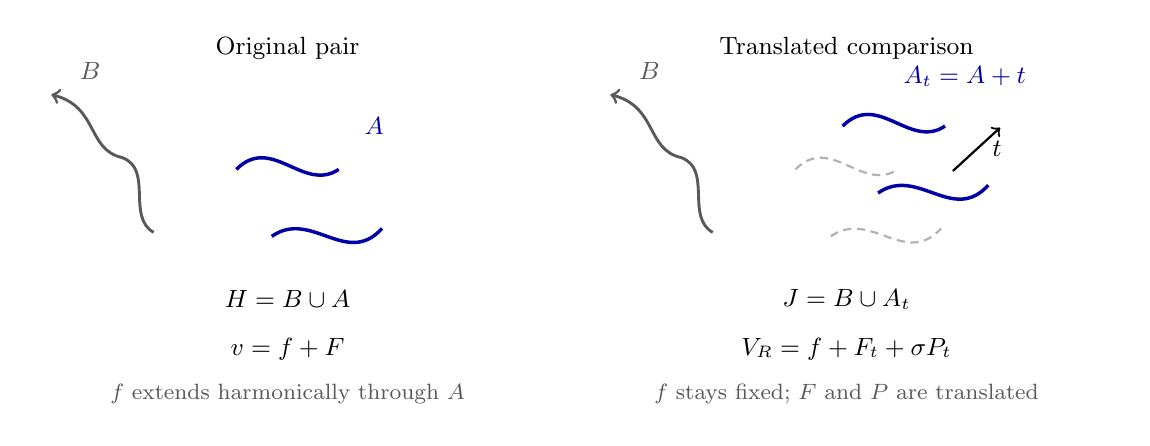
\begin{tikzpicture}[x=1cm,y=1cm,
      every node/.style={font=\small},
      fixed/.style={draw=black!65,line width=1.05pt},
      moving/.style={draw=blue!65!black,line width=1.25pt},
      old/.style={draw=black!30,line width=.8pt,densely dashed}]
    \path[use as bounding box] (-.05,-1.35) rectangle (13.85,3.6);

    \begin{scope}
      \node[anchor=north] at (3.25,3.6) {Original pair};
      \draw[fixed,<-] (.25,2.75)
        .. controls (.85,2.6) and (.7,2.05) .. (1.15,1.95)
        .. controls (1.55,1.8) and (1.2,1.2) .. (1.55,1.0);
      \node[anchor=east,text=black!65] at (1.0,3.05) {$B$};
      \draw[moving] (2.6,1.8)
        .. controls (3.05,2.25) and (3.45,1.5) .. (3.9,1.8);
      \draw[moving] (3.05,.95)
        .. controls (3.55,1.3) and (4.0,.55) .. (4.45,1.05);
      \node[text=blue!65!black] at (4.35,2.35) {$A$};
      \node at (3.25,.15) {$H=B\cup A$};
      \node at (3.25,-.48) {$v=f+F$};
      \node[font=\footnotesize,text=black!65] at (3.25,-1.05)
        {$f$ extends harmonically through $A$};
    \end{scope}

    \begin{scope}[xshift=7.1cm]
      \node[anchor=north] at (3.25,3.6) {Translated comparison};
      \draw[fixed,<-] (.25,2.75)
        .. controls (.85,2.6) and (.7,2.05) .. (1.15,1.95)
        .. controls (1.55,1.8) and (1.2,1.2) .. (1.55,1.0);
      \node[anchor=east,text=black!65] at (1.0,3.05) {$B$};
      \draw[old] (2.6,1.8)
        .. controls (3.05,2.25) and (3.45,1.5) .. (3.9,1.8);
      \draw[old] (3.05,.95)
        .. controls (3.55,1.3) and (4.0,.55) .. (4.45,1.05);
      \begin{scope}[shift={(.6,.55)}]
        \draw[moving] (2.6,1.8)
          .. controls (3.05,2.25) and (3.45,1.5) .. (3.9,1.8);
        \draw[moving] (3.05,.95)
          .. controls (3.55,1.3) and (4.0,.55) .. (4.45,1.05);
      \end{scope}
      \draw[->,line width=.8pt] (4.6,1.78) -- (5.2,2.33)
        node[midway,right=2pt] {$t$};
      \node[text=blue!65!black] at (4.75,2.98) {$A_t=A+t$};
      \node at (3.25,.15) {$J=B\cup A_t$};
      \node at (3.25,-.48) {$V_R=f+F_t+\sigma P_t$};
      \node[font=\footnotesize,text=black!65] at (3.25,-1.05)
        {$f$ stays fixed; $F$ and $P$ are translated};
    \end{scope}
  \end{tikzpicture}
  \caption{The comparison associated with a hypothetical separated compact
  piece $A$.  The remainder $B$ is fixed, while $A$ is translated by a small
  vector $t$ with $A_t\cap B=\varnothing$; the dashed curves mark its former
  position.  The displayed formula for $V_R$ holds in the inner comparison
  disk.  Far away, a cutoff returns the function to $v$.  The drawings are
  schematic: $A$ may contain several components, and no regularity of all of
  $A$ or $B$ is asserted.  The functions $F$ and $P$ need not have compact
  support.}
  \label{fig:compact-translation}
\end{figure}


All hypotheses of Lemmas~\ref{lem:translated-comparison}
and~\ref{lem:harmonic-interaction} now hold. In particular,
\eqref{eq:constant-interactions} holds for every compactly supported
$h'\in W^{1,2}(\mathbb R^2\setminus A)$.

We explain how to remove the projected potential from these interactions.
Let $\phi'$ be the normalized potential associated with such an $h'$.
Since $\operatorname{div}G=0$, testing with $\theta_R\phi'_t$, where
$\theta_R$ is a smooth cutoff on $B_{2R}$ equal to one on $B_R$, gives
\[
 \int\theta_R G\cdot\nabla\phi'_t
       =-\int G\cdot\nabla\theta_R\,\phi'_t.
\]
The compactly supported Sobolev test is justified by smooth approximation,
because $G\in L^2_{\mathrm{loc}}$. By the exterior normalization
$\phi'_t=O(R^{-1})$ on the cutoff annulus and
\eqref{eq:external-field-growth}, the right side is $O(R^{-1/2})$.
The uncut left integrand is absolutely integrable by the same dyadic
estimate used in Lemma~\ref{lem:translated-comparison}. Hence
\begin{equation}
 \int_{\mathbb R^2}G\cdot\nabla\phi'_t=0,
 \qquad
 I_q(t)=\int_{\mathbb R^2}G\cdot(\nabla h')_t.
 \label{eq:remove-projection}
\end{equation}
This step uses the distributional equation and decay, not a claim that
$G$ belongs to global $L^2$.

Take a smaller part of the regular arc in $A$. After a rigid change of
coordinates, it has the form
\[
 \gamma(s)=(s,\kappa(s)),\qquad s\in I,
\]
where $I$ is a bounded interval and $\kappa$ is $C^1$ on a neighborhood of
$\overline I$. Choose $I$ and $a>0$ so that the graph strip
$\{(s,\kappa(s)+r):s\in I,\ |r|<a\}$ is relatively compact in $O$
and meets $H$ only in the continuation of this arc. Let $n(s)$ be one
of its continuous unit normals. Choose
$\eta\in C_c^\infty((-a,a))$ with $\eta(0)=1$.
For every $\beta\in C_c^\infty(I)$ define, on the strip,
\[
 h'_\beta(x_1,x_2)
   =\mathbf 1_{\{x_2>\kappa(x_1)\}}\,
        \beta(x_1)\eta(x_2-\kappa(x_1)),
\]
and extend it by zero outside the strip. Its support avoids the ends
and the outer edge of the strip. Since $\kappa$ is $C^1$, this function is
Sobolev on each side, has its only jump on $A$, and belongs to
$W^{1,2}(\mathbb R^2\setminus A)$. Its trace difference on the arc
is $\beta$. Thus only $C^1$ regularity of the arc is needed. Denote by
$q_\beta$ the field associated with $h'_\beta$ by
Lemma~\ref{lem:compact-projection}.

Decrease the translation disk once so that every translate of this
fixed strip stays in $O$. Integration by parts on its translated upper
side, where $f$ is harmonic, and \eqref{eq:remove-projection} give
\begin{equation}
 I_{q_\beta}(t)
   =\pm\int_I\beta(s)\,
       n(s)\cdot\nabla f(\gamma(s)+t)\,|\gamma'(s)|\,ds.
 \label{eq:jump-flux}
\end{equation}
There are no other boundary terms, because the test vanishes near all
other edges. Translation preserves the normal $n(s)$.

By \eqref{eq:constant-interactions}, the left side of
\eqref{eq:jump-flux} is independent of $t$, for every $\beta$.
The fundamental lemma for tests on $I$ and continuity imply
\[
 n(s)\cdot\nabla f(\gamma(s)+t)
      =n(s)\cdot\nabla f(\gamma(s))
       \qquad(s\in I, |t|<\delta).
\]
Fix an interior $s_0$. A single fixed directional derivative of $f$
is constant on a disk about $\gamma(s_0)$. In two dimensions this
forces a harmonic function to be affine there: in rotated coordinates
$\partial_1 f=c$ gives $f=cx_1+a(x_2)$, and $\Delta f=0$ gives
$a''=0$. Unique continuation for harmonic functions makes $f$ affine
on the connected open set $O$.

Thus $G$ is a constant vector almost everywhere in the plane.
The growth estimate \eqref{eq:external-field-growth} forces that vector
to be zero. Now take $h'=h$, so $q=p$, in
\eqref{eq:constant-interactions}. It gives $\|p\|_2^2=0$.
Consequently $m=G+p=0$ almost everywhere on $D$. Since $D$ is connected,
$v$ is constant there. Extend this constant across $A$ and use the closed rectifiable set
$B$. This is an admissible comparison supported on the compact set $A$:
the function agrees with $v$ almost everywhere, the Dirichlet energy
is unchanged, and the length decreases by $\mathcal H^1(A)>0$.
This contradicts absolute minimality.
\end{proof}

\section{Classification and interior regularity}
\label{sec:assembly}

We now pass from the exclusion of compact pieces to the local geometry of the
original singular set.  The only limiting sets still available will be the
three models in the epsilon-regularity theorem.

\begin{corollary}[Classification of the generalized limits]
\label{cor:classification}
The closed set of every global generalized minimizer arising from absolute
minimizers is empty, a line, a $120$-degree triod of half-lines, or a half-line.
\end{corollary}

\begin{proof}
Let $(v,H,\{p_{kl}\})$ be such a minimizer.  If $H$ disconnects the plane,
Proposition~\ref{prop:planar-facts}(\ref{item:classification}) gives the
conclusion.  Otherwise Proposition~\ref{prop:planar-facts}(\ref{item:connected-absolute})
gives absolute minimality.  If $H$ had a bounded component,
Lemma~\ref{lem:compact-isolation} would enclose it in a separated compact
piece $A$ of positive length.  Its length measure is concentrated on points
with arc neighborhoods, by
Proposition~\ref{prop:planar-facts}(\ref{item:global-estimates}), so one such
arc lies in $A$.  Proposition~\ref{prop:compact-piece} rules out this piece.
Thus $H$ has no bounded component, while
Proposition~\ref{prop:planar-facts}(\ref{item:classification}) allows at most
one unbounded component.  Hence $H$ is empty or connected.  In either case all but
at most one component lie in a compact set, so the remaining classification
statement in that proposition applies.
\end{proof}

\begin{proof}[Completion of the proof of Theorem~\ref{thm:main}]
Proposition~\ref{prop:initial-reduction} allows us to apply
Proposition~\ref{prop:planar-facts}.  Fix $x\in K$ and take a blow-up with
limiting set $H$.  Since $0\in H$, Corollary~\ref{cor:classification} leaves
three possibilities: a line, a half-line, or a triod of half-lines.
Choose $\rho>0$ so that in $B_{3\rho}(0)$ the limiting set is a model centered
at zero.  If the vertex of a half-line or triod is different from zero, it
suffices to take $3\rho$ less than its distance from zero; the model is then a
line.

Local bilateral Hausdorff convergence gives
\[
 \operatorname{dist}_{\mathrm H}
 \bigl(K_j\cap B_{2\rho}(0),H\cap B_{2\rho}(0)\bigr)=o(\rho).
\]
To justify truncation at the sphere, move each model point near
$\partial B_{2\rho}$ slightly inward along its ray, apply convergence in
$B_{3\rho}$, and then let the inward displacement tend to zero.  Approximating
points are now inside $B_{2\rho}$; the reverse distance follows by the same
radial projection onto the truncated model.

Put $s_j=r_j\rho$ and return to the original coordinates.  For large $j$, the
closed set in $B_{2s_j}(x)$ has model distance $o(s_j)$, the enlarged ball is
compactly contained in the original domain, and $s_j\leq1$.  The fixed-data
epsilon-regularity statement
Proposition~\ref{prop:planar-facts}(\ref{item:epsilon}) now applies to the
original minimizer.  It follows that the entire set $K\cap B_{s_j}(x)$ is
$C^{1,\alpha}$-diffeomorphic to the corresponding model.

The endpoint or triple junction in this chart may have shifted from its
center.  This causes no difficulty: $x$ is either an interior point of one of
the arcs or the actual endpoint or junction.  Restricting the chart around
$x$ gives its corresponding local model.  The equal-angle conclusion for a
triple junction is part of the epsilon-regularity theorem.  We have therefore
proved the asserted interior regularity at every point of $K$.

It remains to prove local finiteness of the global connected components.
For each $x\in K$, retain one of the original epsilon-regularity disks
$B_{s_x}(x)\Subset\Omega$, whose entire intersection with $K$ is connected.
If $U\Subset\Omega$ is open, then
$K\cap\overline U$ is compact, so finitely many of these disks cover it.
Each disk meets only one global connected component of $K$, because its entire
intersection with $K$ is connected.  Every global component meeting $U$
therefore belongs to the finite list represented by the covering disks.
\end{proof}

\begin{remark}[Local scope]
The local models also make the endpoints and triple junctions a relatively
closed discrete subset of $K$, so only finitely many of them meet a compact
subset of $\Omega$.  Define the edges to be the connected components left
after deleting these endpoints and triple junctions from $K$.  In each model
chart, deleting those points leaves at most three connected pieces, each
contained in one global edge.  A finite model-chart cover therefore meets only
finitely many global edges.  These are interior finiteness statements, with
no assertion at $\partial\Omega$.  They concern global components rather than
components of $K\cap U$: even one straight line can have infinitely many
intersection components with an arbitrary relatively compact open set.
\end{remark}

The geometric conclusion also gives an endpoint integrability estimate for
the gradient.  Its exponent is suggested by the crack-tip profile
$r^{1/2}\sin(\theta/2)$: the gradient has size proportional to $r^{-1/2}$,
so its superlevel sets near the tip have area of order $t^{-4}$ for large
$t$, whereas its fourth power is not locally integrable
\cite[Section~1.4]{delellis_focardi2025}.  The next result gives this
weak-$L^4$ bound for every minimizer in Theorem~\ref{thm:main}, using the
De Lellis--Focardi equivalence between the absence of irregular points and
the weak-$L^4$ estimate.

\begin{corollary}[Local weak-$L^4$ gradient bound]\label{cor:weak-l4}
Let $(u,K)$ satisfy the hypotheses of Theorem~\ref{thm:main}.
Let $\nabla u$ denote the approximate gradient furnished by
Proposition~\ref{prop:initial-reduction}; it agrees almost everywhere on
$\Omega\setminus K$ with the gradient in \eqref{eq:original-energy}.
For every open $U\Subset\Omega$ there is a constant $C_U<\infty$,
depending on $U$ and the minimizer, such that
\begin{equation}\label{eq:weak-l4}
 \mathcal L^2\bigl(\{x\in U\setminus K:|\nabla u(x)|>t\}\bigr)
 \le C_Ut^{-4}\qquad\text{for every }t>0,
\end{equation}
where $\mathcal L^2$ denotes planar Lebesgue measure. In particular,
$\nabla u\in L^{4,\infty}_{\mathrm{loc}}(\Omega)$ and
$\nabla u\in L^p_{\mathrm{loc}}(\Omega)$ for every $0<p<4$.
\end{corollary}

\begin{proof}
Fix $U\Subset\Omega$ and choose a smooth open set $W$ with
$U\Subset W\Subset\Omega$. Proposition~\ref{prop:initial-reduction}
makes the restricted pair a reduced rectifiable absolute minimizer for
the energy $E_1$ of De Lellis--Focardi, with bounded fidelity datum.
The three models in Theorem~\ref{thm:main} are precisely their regular
pure-jump, loose-end, and triple-junction models: the arcs can be
straightened to their tangent rays by a $C^1$ chart tangent to the
identity at the center, and the triple angles are $120$ degrees
\cite[Definitions~1.3.2 and~1.5.1]{delellis_focardi2025}.
Thus the irregular stratum $K^{(i)}$ of the restricted pair is empty.
Their weak-$L^4$ equivalence
\cite[Theorem~1.5.4; see also Theorem~6.1.6]{delellis_focardi2025}
gives the superlevel estimate \eqref{eq:weak-l4} on $U$, after increasing
$C_U$ for $0<t<1$. Since $\mathcal H^1(K)<\infty$ implies
$\mathcal L^2(K)=0$, this is also the weak-$L^4$ bound for the approximate
gradient. For $0<p<4$, the layer-cake formula bounds
$\int_U|\nabla u|^p\,dx$ by
\[
 p\int_0^\infty t^{p-1}
   \min\{\mathcal L^2(U),C_Ut^{-4}\}\,dt<\infty.
\]
\end{proof}

\begingroup
\small
\bibliographystyle{plain}
\bibliography{references}
\endgroup
\end{document}
